\section{线性表 (Linear  List)}

\begin{frame}[fragile]
  \frametitle{线性表 --- Linear  List}
  \begin{enumerate}
  \item 基本概念
  \item 顺序表
  \item 链表
  \end{enumerate}
\end{frame}

\subsection{线性表概述}
\begin{frame}[fragile]
  \frametitle{线性表}

  \begin{easylist}
    & 线性表举例:
    && 英文字母表 $A, B, C, \cdots, Z$
    && 某单位近5年的计算机数量 $(40, 60, 100, 150, 180)$
    && 某产品淘宝的销售记录.
    
    & 特点
    && 数据元素是多样的,但具有相同特性
    && 相邻元素之间有序偶关系<前驱, 后继>    
  \end{easylist}
\end{frame}

\begin{frame}[fragile]
  \frametitle{线性表}

  \begin{tcolorbox}[standard jigsaw, opacityback=0, colframe=red, title=线性表是n个数据元素的有限序列]
    \[
    (a_1, a_2, \cdots, a_i, \cdots, a_n)
    \]
  \end{tcolorbox}

  \begin{itemize}
  \item 存在唯一的{\color{red}第一个}数据元素,存在唯一的的{\color{red}最后一个}数据元素。
  \item 除第一个之外,每个数据元素只有一个前驱;除最后一个之外,每个数据元素只有
    一个后继。
  \item 线性表的长度:线性表中元素的个数,常记作length, len, n. 当空表时,len=0.
  \end{itemize}
\end{frame}

\begin{frame}[fragile]
  \frametitle{线性表的两种存储方式}
  \begin{enumerate}
  \item 方案1:顺序存储 --- 称顺序表
  \item 方案2:链式存储 --- 称链表
  \end{enumerate}
\end{frame}


\subsection{顺序表}
\begin{frame}[fragile]
  \frametitle{方案1: 顺序表 (Sequence List)}
  \begin{columns}
    \begin{column}[T]{.5\linewidth}
      \[
      (a_1, a_2, \cdots, a_i, \cdots, a_n)
      \]
      \begin{easylist}
        & 建一个数组, 用一组地址连续的存储单元依次存储数据元素。

        && 逻辑上相邻的数据元素,其物理存储位置也相邻

      \end{easylist}
    \end{column}
    \begin{column}[T]{.5\linewidth}
      \begin{tcolorbox}[]
        \scalebox{0.7}{
          \begin{tikzpicture}[scale=0.5, box/.style={draw, minimum width=1.2cm, minimum height=0.5cm, fill=yellow!10}]
	          \draw node[box] (a1) {$a_1$}
	          node[box, below=0 of a1] (a2) {$a_2$}
	          node[box, below=0 of a2] (a3) {$\cdots$}
	          node[box, below=0 of a3] (ai) {$a_i$}
	          node[box, below=0 of ai] (a5) {$\cdots$}
	          node[box, below=0 of a5] (an) {$a_n$}
	          node[box, below=0 of an, fill=gray!30] (a7) {}
	          node[box, below=0 of a7, fill=gray!30] (a8) {}
	          node[box, below=0 of a8, fill=gray!30] (a9) {};

	          \draw node[right=0.3 of a1] (p1) {$1$}
	          node[right=0.3 of a2] (p2) {$2$}
	          node[right=0.3 of ai] (pi) {$i$}
	          node[right=0.3 of an] (pn) {$n$}
	          node[right=0.3 of a7] (p7) {空闲}
	          node[right=0.3 of a8] (p8) {空闲}
	          node[right=0.3 of a9] (p9) {空闲};

	          \draw node[left=0.3 of a1] (p1) {$b$}
	          node[left=0.3 of a2] (p2) {$b+l$}
	          node[left=0.3 of ai] (pi) {$b+(i-1)\cdot l$}
	          node[left=0.3 of an] (pn) {$b+(n-1)\cdot l$}
	          node[left=0.3 of a7] (p7) {$b+n\cdot l$}
	          node[left=0.3 of a8] (p8) {$\cdots$}
	          node[left=0.3 of a9] (p9) {$b+(MaxLen-1)\cdot l$};

	          \draw node[above left=0.3 of p1] (tip) {起始地址/基地址};
	          \draw[draw=red, thick, -Latex] (tip) -> (p1);
          \end{tikzpicture}
        }
      \end{tcolorbox}
    \end{column}
  \end{columns}
\end{frame}

\begin{frame}[fragile]
  \frametitle{顺序表 (Sequence List)}
  \begin{columns}
    \begin{column}[T]{.5\linewidth}
      \begin{easylist}
        & 为便于维护处理,记录3个变量
        && 存放表元素的数组list;
        && 表的长度length;
        && 存储容量maxSize;
        & 常用的基本操作:
        && 判断是否空isEmpty()
        && 求长度 length()
        && 取元素get(i)
        && 插入操作:insert(i,x)
        && 删除操作:remove(i)
        && 查找indexOf(x)
        && 输出display()
      \end{easylist}
    \end{column}
    \begin{column}[T]{.5\linewidth}
      \begin{tcolorbox}[]
        \scalebox{0.7}{
          \begin{tikzpicture}[scale=0.5, box/.style={draw, minimum width=1.2cm, minimum height=0.5cm, fill=yellow!10}]
	          \draw node[box] (a1) {$a_1$}
	          node[box, below=0 of a1] (a2) {$a_2$}
	          node[box, below=0 of a2] (a3) {$\cdots$}
	          node[box, below=0 of a3] (ai) {$a_i$}
	          node[box, below=0 of ai] (a5) {$\cdots$}
	          node[box, below=0 of a5] (an) {$a_n$}
	          node[box, below=0 of an, fill=gray!30] (a7) {}
	          node[box, below=0 of a7, fill=gray!30] (a8) {}
	          node[box, below=0 of a8, fill=gray!30] (a9) {};

	          \draw node[right=0.3 of a1] (p1) {$1$}
	          node[right=0.3 of a2] (p2) {$2$}
	          node[right=0.3 of ai] (pi) {$i$}
	          node[right=0.3 of an] (pn) {$n$}
	          node[right=0.3 of a7] (p7) {空闲}
	          node[right=0.3 of a8] (p8) {空闲}
	          node[right=0.3 of a9] (p9) {空闲};

	          \draw node[left=0.3 of a1] (p1) {$b$}
	          node[left=0.3 of a2] (p2) {$b+l$}
	          node[left=0.3 of ai] (pi) {$b+(i-1)\cdot l$}
	          node[left=0.3 of an] (pn) {$b+(n-1)\cdot l$}
	          node[left=0.3 of a7] (p7) {$b+n\cdot l$}
	          node[left=0.3 of a8] (p8) {$\cdots$}
	          node[left=0.3 of a9] (p9) {$b+(MaxLen-1)\cdot l$};
          \end{tikzpicture}
        }
      \end{tcolorbox}
    \end{column}
  \end{columns}
\end{frame}

\begin{frame}[fragile]
  \frametitle{补充:常用命名规则之驼峰与蛇形命名法}
  \begin{center}
    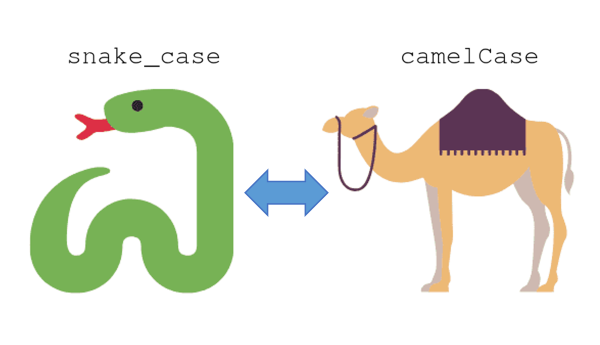
\includegraphics[width=0.5\textwidth]{figs/list/snake_case_camel_case.png}
    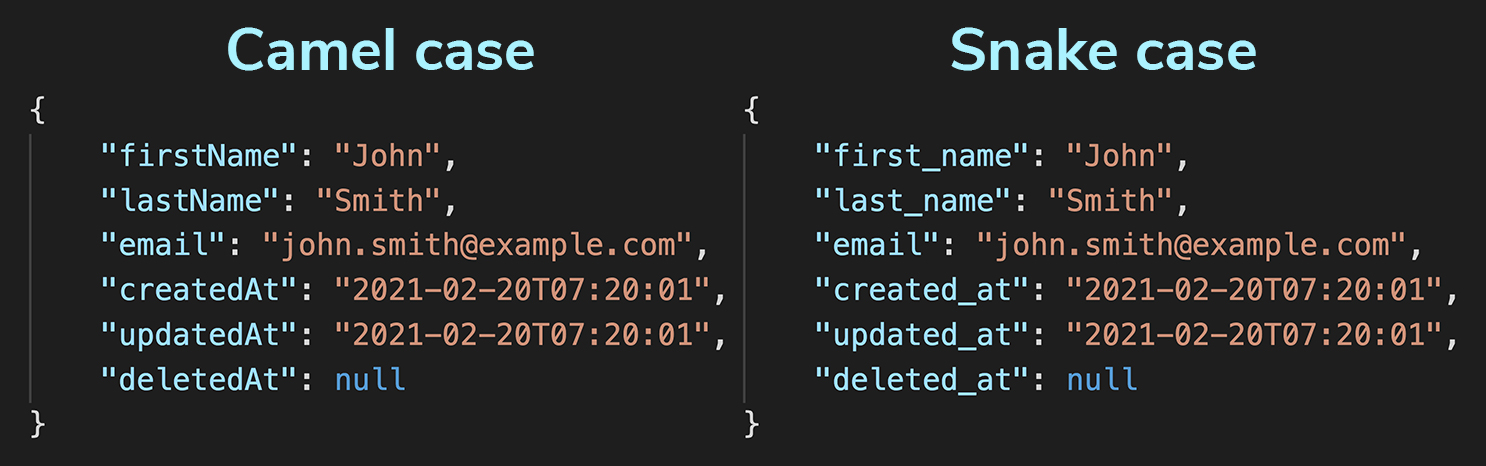
\includegraphics[width=0.85\textwidth]{figs/list/snake_vs_camel.jpg}
  \end{center}
\end{frame}

\begin{frame}[fragile]
  %\frametitle{线性表}
  \begin{minted}{java}
public class SequenceList {
    int maxSize; //最大长度
    int length; //当前长度
    Elem[] list; //对象数组

    public bool isEmpty()
    public int length()
    public Elem get(i) throws Exception
    public void insert(i,e)
    public void remove(i) throws Exception
    public int indexOf(e)
    public void display()
    public void clear()
}
  \end{minted}
\end{frame}

\begin{frame}[fragile]
  %\frametitle{线性表}
  \begin{minted}{python}
class SequenceList:
    def __init__(self, max_size, elements):
        self.max_size = max_size
        self.length = len(elements)
        self.elements = [0]*max_size
        for idx, value in enumerate(elements):
            self.elements[idx] = value

    def __len__(self):
        return self.length

    def __getitem__(self, i):
        return self.elements[i]

    def __setitem__(self, i, value):
        self.elements[i] = value

    def __delitem__(self, i):
        del self.elements[i]
        self.length = self.length - 1
  \end{minted}
\end{frame}

\begin{frame}[fragile]
  \frametitle{初始化顺序表}
  Java/C Example

  \begin{minted}{java}
//初始化空表
void initList(int size) {
    list = new Elem[size];
    maxSize = size; //初始存储容量
    length = 0; //空表长度为0
}
  \end{minted}

  Python Example:

  \begin{minted}{python}
    self.elements = [0]*max_size
  \end{minted}
\end{frame}

\begin{frame}[fragile]
  \frametitle{在index位置上插入元素e}
  \begin{minted}{java}
boolean insert(int index, Elem e) {
  if (length== maxSize)    //当前线性表已满
     {print("顺序表已满!");  return false;}
  if (index < 0 || index > length)    //插入位置编号不合法
    {print("参数错误!");  return false;}

  for (int j = length- 1; j >= index; j--)   //向后移动元素
     list[j + 1] = list[j];

  list[index] = e;    //插入元素
  length ++;
  return true;
}
  \end{minted}
\end{frame}


\begin{frame}[fragile]
  \frametitle{插入元素的时间复杂度}

  \scalebox{0.75} {
    \begin{tikzpicture}[box/.style={draw, minimum width=1.2cm, minimum height=0.65cm, fill=yellow!10}]
	    \draw node[box] (a1) {$a_1$}
	    node[box, right=0 of a1] (a2) {$a_2$}
	    node[box, right=0 of a2] (a3) {$\cdots$}
	    node[box, right=0 of a3] (a4) {$\cdots$}
	    node[box, right=0 of a4] (ai) {$a_i$}
	    node[box, right=0 of ai] (a6) {$\cdots$}
	    node[box, right=0 of a6] (a7) {$\cdots$}
	    node[box, right=0 of a7] (an) {$a_n$}
		  node[draw=red, ellipse, minimum width=0.65cm, minimum height=0.65cm, thick, fill=blue!10, below=0.5 of ai] (cur) {$e$};
		  \draw[draw = red, -Latex] (cur) -- (ai);
    \end{tikzpicture}
  }

  \begin{easylist}
    & 在长为n的线性表中插入一个元素,所需移动元素次数的平均次数为?

    && 有多少种可能的插入位置?$n+1$

    && 假设这些位置以同等概率出现,每个概率$\dfrac{1}{n+1}$。每个情形下分别移动
    $n, n-1, \cdots, 0$次。求加权和为$n/2$。

    && 平均时间复杂度:$T(n)=O(n)$
  \end{easylist}
\end{frame}

\begin{frame}[fragile]
  \frametitle{删除index位置上的元素}
  \scalebox{0.7}{
    \begin{tikzpicture}[scale=0.5, box/.style={draw, minimum width=1.2cm, minimum height=0.65cm, fill=yellow!10}]
	    \draw node[box] (a1) {$a_1$}
	    node[box, right=0 of a1] (a2) {$a_2$}
	    node[box, right=0 of a2] (a3) {$\cdots$}
	    node[box, right=0 of a3] (a4) {$\cdots$}
	    node[box, draw=red, thick, fill=red!20, right=0 of a4] (ai) {$a_i$}
	    node[box, right=0 of ai] (a6) {$\cdots$}
	    node[box, right=0 of a6] (a7) {$\cdots$}
	    node[box, right=0 of a7] (an) {$a_n$};
    \end{tikzpicture}
  }

  \begin{minted}{java}
boolean remove(int index) {
    if(index<0||index>=length)  
          return false;
    if(getLength()==0)
          return false;
    for (int j=index;j<length-1; j++)    //前移
          Elem[j]=elem[j+1];
    length--;
}
  \end{minted}
\end{frame}

\begin{frame}[fragile]
  \frametitle{删除元素的时间复杂度}
  \scalebox{0.7}{
    \begin{tikzpicture}[scale=0.5, box/.style={draw, minimum width=1.2cm, minimum height=0.65cm, fill=yellow!10}]
	    \draw node[box] (a1) {$a_1$}
	    node[box, right=0 of a1] (a2) {$a_2$}
	    node[box, right=0 of a2] (a3) {$\cdots$}
	    node[box, right=0 of a3] (a4) {$\cdots$}
	    node[box, draw=red, thick, fill=red!20, right=0 of a4] (ai) {$a_i$}
	    node[box, right=0 of ai] (a6) {$\cdots$}
	    node[box, right=0 of a6] (a7) {$\cdots$}
	    node[box, right=0 of a7] (an) {$a_n$};
    \end{tikzpicture}
  }

  \begin{itemize}
  \item 在长度为n的线性表中删除一个元素:
    \begin{itemize}
    \item 共有n个可能的位置,每个有1/n的概率。每个情形下分别移动n-1, …, 0次。求加权和为(n-1)/2。
    \item $T(n)=O(n)$
    \end{itemize}
  \end{itemize}

  \pause

  \begin{tcolorbox}[standard jigsaw, opacityback=0, colframe=red, title=结论]
    在顺序表中插入或删除一个元素时,平均移动一半元素,当$n$很大时,效率很低.
  \end{tcolorbox}
\end{frame}

\begin{frame}[fragile]
  \frametitle{顺序表特点:地址连续}
  \begin{columns}
    \begin{column}[T]{.5\linewidth}
      \begin{tcolorbox}[]
      \scalebox{0.7}{
        \begin{tikzpicture}[scale=0.5, box/.style={draw, minimum width=1.2cm, minimum height=0.5cm, fill=yellow!10}]
	        \draw node[box] (a1) {$a_1$}
	        node[box, below=0 of a1] (a2) {$a_2$}
	        node[box, below=0 of a2] (a3) {$\cdots$}
	        node[box, below=0 of a3] (ai) {$a_i$}
	        node[box, below=0 of ai] (a5) {$\cdots$}
	        node[box, below=0 of a5] (an) {$a_n$}
	        node[box, below=0 of an, fill=gray!30] (a7) {}
	        node[box, below=0 of a7, fill=gray!30] (a8) {}
	        node[box, below=0 of a8, fill=gray!30] (a9) {};

	        \draw node[right=0.3 of a1] (p1) {$1$}
	        node[right=0.3 of a2] (p2) {$2$}
	        node[right=0.3 of ai] (pi) {$i$}
	        node[right=0.3 of an] (pn) {$n$}
	        node[right=0.3 of a7] (p7) {空闲}
	        node[right=0.3 of a8] (p8) {空闲}
	        node[right=0.3 of a9] (p9) {空闲};

	        \draw node[left=0.3 of a1] (p1) {$b$}
	        node[left=0.3 of a2] (p2) {$b+l$}
	        node[left=0.3 of ai] (pi) {$b+(i-1)\cdot l$}
	        node[left=0.3 of an] (pn) {$b+(n-1)\cdot l$}
	        node[left=0.3 of a7] (p7) {$b+n\cdot l$}
	        node[left=0.3 of a8] (p8) {$\cdots$}
	        node[left=0.3 of a9] (p9) {$b+(MaxLen-1)\cdot l$};
        \end{tikzpicture}
      }
      \end{tcolorbox}
    \end{column}
    \begin{column}[T]{.5\linewidth}
      \begin{easylist}
        & 优点
        && 直观
        && 随机存储效率高
        \pause
        & 缺点
        && 移动元素代价大
      \end{easylist}
    \end{column}
  \end{columns}
\end{frame}


\subsection{链表}
\begin{frame}[fragile]
  \frametitle{方案2: 链式存储---链表}
  \begin{columns}
    \begin{column}[T]{.4\linewidth}
      \scalebox{0.5}{    \begin{tikzpicture}[fill=red, box/.style={draw, minimum width=2cm, minimum height=0.85cm, fill=yellow!10}]
	      \draw node[box] (dh) {数据域}  node[box, right=0 of dh] (ph) {指针域}
	 node[box, below=0.5 of dh] (d_li) {LI}  node[box, right=0 of d_li] (p_li) {43} node[left=0.2 of d_li] {1}
	 node[box, below=0.5 of d_li] (d_qian) {QIAN}  node[box, right=0 of d_qian] (p_qian) {13} node[left=0.2 of d_qian] {7}
	 node[box, below=0.5 of d_qian] (d_sun) {SUN}  node[box, right=0 of d_sun] (p_sun) {1} node[left=0.2 of d_sun] {13}
	 node[box, below=0.5 of d_sun] (d_wang) {WANG}  node[box, right=0 of d_wang] (p_wang) {?} node[left=0.2 of d_wang] {19}
	 node[box, below=0.5 of d_wang] (d_wu) {WU}  node[box, right=0 of d_wu] (p_wu) {37} node[left=0.2 of d_wu] {25}
	 node[box, below=0.5 of d_wu] (d_zhao) {ZHAO}  node[box, right=0 of d_zhao] (p_zhao) {7} node[left=0.2 of d_zhao] {31}
	 node[box, below=0.5 of d_zhao] (d_zheng) {ZHENG}  node[box, right=0 of d_zheng] (p_zheng) {?} node[left=0.2 of d_zheng] {37}
	 node[box, below=0.5 of d_zheng] (d_zhou) {ZHOU}  node[box, right=0 of d_zhou] (p_zhou) {25} node[left=0.2 of d_zhou] {43}
	node[box, minimum width=0.85cm, draw=red, fill=red!20, left=1 of d_li] (h) {31};

	\path[draw=red] (h.center) edge[out=270, in=155, -Latex, draw=red, thick] (d_zhao.west);
	\path[draw=blue] (p_zhao.east) edge[out=0, in=225, -Latex] (d_qian.west);
	\path[draw=blue] (p_qian.east) edge[out=0, in=225, -Latex] (d_sun.west);
	\path[draw=blue] (p_sun.east) edge[out=0, in=225, -Latex] (d_li.west);
\end{tikzpicture}

}
    \end{column}
    \begin{column}[T]{.6\linewidth}
      用一组任意的存储单元存储线性表的数据元素,利用指针指向直接后继的存储位置
    \end{column}
  \end{columns}
\end{frame}

\begin{frame}[fragile]
  \frametitle{单链表的类型定义}
  \begin{columns}
    \begin{column}[T]{.4\linewidth}
      \scalebox{0.5}{    \begin{tikzpicture}[fill=red, box/.style={draw, minimum width=2cm, minimum height=0.85cm, fill=yellow!10}]
	      \draw node[box] (dh) {数据域}  node[box, right=0 of dh] (ph) {指针域}
	 node[box, below=0.5 of dh] (d_li) {LI}  node[box, right=0 of d_li] (p_li) {43} node[left=0.2 of d_li] {1}
	 node[box, below=0.5 of d_li] (d_qian) {QIAN}  node[box, right=0 of d_qian] (p_qian) {13} node[left=0.2 of d_qian] {7}
	 node[box, below=0.5 of d_qian] (d_sun) {SUN}  node[box, right=0 of d_sun] (p_sun) {1} node[left=0.2 of d_sun] {13}
	 node[box, below=0.5 of d_sun] (d_wang) {WANG}  node[box, right=0 of d_wang] (p_wang) {?} node[left=0.2 of d_wang] {19}
	 node[box, below=0.5 of d_wang] (d_wu) {WU}  node[box, right=0 of d_wu] (p_wu) {37} node[left=0.2 of d_wu] {25}
	 node[box, below=0.5 of d_wu] (d_zhao) {ZHAO}  node[box, right=0 of d_zhao] (p_zhao) {7} node[left=0.2 of d_zhao] {31}
	 node[box, below=0.5 of d_zhao] (d_zheng) {ZHENG}  node[box, right=0 of d_zheng] (p_zheng) {?} node[left=0.2 of d_zheng] {37}
	 node[box, below=0.5 of d_zheng] (d_zhou) {ZHOU}  node[box, right=0 of d_zhou] (p_zhou) {25} node[left=0.2 of d_zhou] {43}
	node[box, minimum width=0.85cm, draw=red, fill=red!20, left=1 of d_li] (h) {31};

	\path[draw=red] (h.center) edge[out=270, in=155, -Latex, draw=red, thick] (d_zhao.west);
	\path[draw=blue] (p_zhao.east) edge[out=0, in=225, -Latex] (d_qian.west);
	\path[draw=blue] (p_qian.east) edge[out=0, in=225, -Latex] (d_sun.west);
	\path[draw=blue] (p_sun.east) edge[out=0, in=225, -Latex] (d_li.west);
\end{tikzpicture}

}
    \end{column}
    \begin{column}[T]{.6\linewidth}
      \begin{easylist}
        & 单链表:每个结点有一个指针域
        & 单链表可由头指针唯一确定,头指针指向第一个结点。
        & Java Code:

        \scriptsize

        \begin{minted}{java}
          class Node {
            Object data;
            Node next;
          }
        \end{minted}

      \end{easylist}
    \end{column}
  \end{columns}
\end{frame}

\begin{frame}[fragile]
  \frametitle{单链表的类型定义}
  \begin{columns}
    \begin{column}[T]{.4\linewidth}
      \scalebox{0.5}{    \begin{tikzpicture}[fill=red, box/.style={draw, minimum width=2cm, minimum height=0.85cm, fill=yellow!10}]
	      \draw node[box] (dh) {数据域}  node[box, right=0 of dh] (ph) {指针域}
	 node[box, below=0.5 of dh] (d_li) {LI}  node[box, right=0 of d_li] (p_li) {43} node[left=0.2 of d_li] {1}
	 node[box, below=0.5 of d_li] (d_qian) {QIAN}  node[box, right=0 of d_qian] (p_qian) {13} node[left=0.2 of d_qian] {7}
	 node[box, below=0.5 of d_qian] (d_sun) {SUN}  node[box, right=0 of d_sun] (p_sun) {1} node[left=0.2 of d_sun] {13}
	 node[box, below=0.5 of d_sun] (d_wang) {WANG}  node[box, right=0 of d_wang] (p_wang) {?} node[left=0.2 of d_wang] {19}
	 node[box, below=0.5 of d_wang] (d_wu) {WU}  node[box, right=0 of d_wu] (p_wu) {37} node[left=0.2 of d_wu] {25}
	 node[box, below=0.5 of d_wu] (d_zhao) {ZHAO}  node[box, right=0 of d_zhao] (p_zhao) {7} node[left=0.2 of d_zhao] {31}
	 node[box, below=0.5 of d_zhao] (d_zheng) {ZHENG}  node[box, right=0 of d_zheng] (p_zheng) {?} node[left=0.2 of d_zheng] {37}
	 node[box, below=0.5 of d_zheng] (d_zhou) {ZHOU}  node[box, right=0 of d_zhou] (p_zhou) {25} node[left=0.2 of d_zhou] {43}
	node[box, minimum width=0.85cm, draw=red, fill=red!20, left=1 of d_li] (h) {31};

	\path[draw=red] (h.center) edge[out=270, in=155, -Latex, draw=red, thick] (d_zhao.west);
	\path[draw=blue] (p_zhao.east) edge[out=0, in=225, -Latex] (d_qian.west);
	\path[draw=blue] (p_qian.east) edge[out=0, in=225, -Latex] (d_sun.west);
	\path[draw=blue] (p_sun.east) edge[out=0, in=225, -Latex] (d_li.west);
\end{tikzpicture}

}
    \end{column}
    \begin{column}[T]{.6\linewidth}
      \begin{easylist}
        & 单链表:每个结点有一个指针域
        & 单链表可由头指针唯一确定,头指针指向第一个结点。
        & Python Code:
        \scriptsize

        \begin{minted}{python}
          class Node:
            def __init__(self, data, next=None):
              self.data = data
              self.next = next

          first = Node(1)
          second = Node(2)
          last = Node(3)
          first.next=second
          second.next = last
          print(first.next.next.data)
        \end{minted}

      \end{easylist}
    \end{column}
  \end{columns}
\end{frame}

\begin{frame}[fragile]
  \frametitle{单链表上的常见操作}
  \begin{enumerate}
  \item 建立单链表create()
  \item 求表长length()
  \item 查找index(value)
  \item 插入insert(i,e)
  \item 删除remove(i)
  \item 获取元素get(index)
  \item 显示display()
  \end{enumerate}
\end{frame}

\begin{frame}[fragile]
  \frametitle{建立单链表}
  \begin{itemize}
  \item 链表是{\color{red}动态管理}的:链表中的每个结点占用的存储空间不是预先分
    配,而是运行时系统根据需求而生成的。
  \item 建立单链表从空表开始,每读入一个数据元素则申请一个结点,插入链表。
  \end{itemize}
\end{frame}

\begin{frame}[fragile]
  \frametitle{建立单链表:两种不同方式}
  如依次读入  25, 45, 18…

  \begin{columns}
    \begin{column}[T]{.5\linewidth}
      头部插入:

      \scalebox{0.5}{
        \begin{tikzpicture}[fill=red, box/.style={draw, minimum width=0.85cm, minimum height=0.8cm, fill=red!5}]
	        \draw node[box] (h) {$\wedge$};

	        \draw node[box, below=0.5 of h] (h) {} node[box, right=of h] (d25) {25}  node[box, right=0 of d25] (p25) {$\wedge$};
	        \draw[draw, -Latex] (h.center) -- (d25);

	        \draw node[box, below=0.5 of h] (h) {}
          node[box, right=of h] (d45) {45}  node[box, right=0 of d45] (p45) {}
          node[box, right=of p45] (d25) {25}  node[box, right=0 of d25] (p25) {$\wedge$};
	        \draw[draw, -Latex] (h.center)  edge[-latex] (d45) (p45.center) -- (d25);

	        \draw node[box, below=0.5 of h] (h) {}
          node[box, right=of h] (d18) {18}  node[box, right=0 of d18] (p18) {}
          node[box, right=of p18] (d45) {45}  node[box, right=0 of d45] (p45) {}
          node[box, right=of p45] (d25) {25}  node[box, right=0 of d25] (p25) {$\wedge$};
	        \path[draw, -Latex] (h.center) edge[-latex] (d18) (p18.center)  edge[-latex] (d45)  (p45.center) -- (d25);
        \end{tikzpicture}
      }
    \end{column}
    \begin{column}[T]{.5\linewidth}
      尾部插入:

      \scalebox{0.5}{
        \begin{tikzpicture}[fill=red, box/.style={draw, minimum width=0.85cm, minimum height=0.8cm, fill=red!5}]
	        \draw node[box] (h) {$\wedge$};

	        \draw node[box, below=0.5 of h] (h) {} node[box, right=of h] (d25) {25}  node[box, right=0 of d25] (p25) {$\wedge$};
	        \draw[draw, -Latex] (h.center) -- (d25);

	        \draw node[box, below=0.5 of h] (h) {}
          node[box, right=of h] (d45) {25}  node[box, right=0 of d45] (p45) {}
          node[box, right=of p45] (d25) {45}  node[box, right=0 of d25] (p25) {$\wedge$};
	        \draw[draw, -Latex] (h.center)  edge[-latex] (d45) (p45.center) -- (d25);

	        \draw node[box, below=0.5 of h] (h) {}
          node[box, right=of h] (d18) {25}  node[box, right=0 of d18] (p18) {}
          node[box, right=of p18] (d45) {45}  node[box, right=0 of d45] (p45) {}
          node[box, right=of p45] (d25) {18}  node[box, right=0 of d25] (p25) {$\wedge$};
	        \path[draw, -Latex] (h.center) edge[-latex] (d18) (p18.center)  edge[-latex] (d45)  (p45.center) -- (d25);
        \end{tikzpicture}
      }
    \end{column}
  \end{columns}
\end{frame}

\subsection{作业}
\begin{frame}[fragile]
  \frametitle{约瑟夫环}

  在罗马人占领乔塔帕特后,约瑟夫及他的40个战友躲到一个洞中,这些犹太人宁死也不想
  被敌人抓到,于是决定了一个自杀方式:

  \begin{itemize}
    \item 41个人排成一个圆圈,由第1个人开始报数,每报数到第3人该人就必须自杀,然
      后再由下一个重新报数,直到所有人都自杀身亡为止。
  \item 约瑟夫说他和另一个人逃过了这场死亡游戏: by luck or by the hand of God.
  \item 请问约瑟夫在这个圆圈中的位置是?
  \end{itemize}
\end{frame}

\begin{frame}[fragile]
  \frametitle{约瑟夫环}

  \begin{columns}
    \begin{column}[T]{.5\linewidth}
      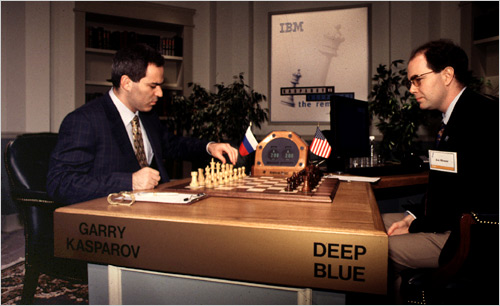
\includegraphics[width=0.8\textwidth]{figs/intro/deep_blue_1.png}

        1997年5月11日,国际象棋世界冠军卡斯帕罗夫与IBM公司的超级电脑深蓝(Deep Blue)对弈。
    \end{column}
    \begin{column}[T]{.5\linewidth}
      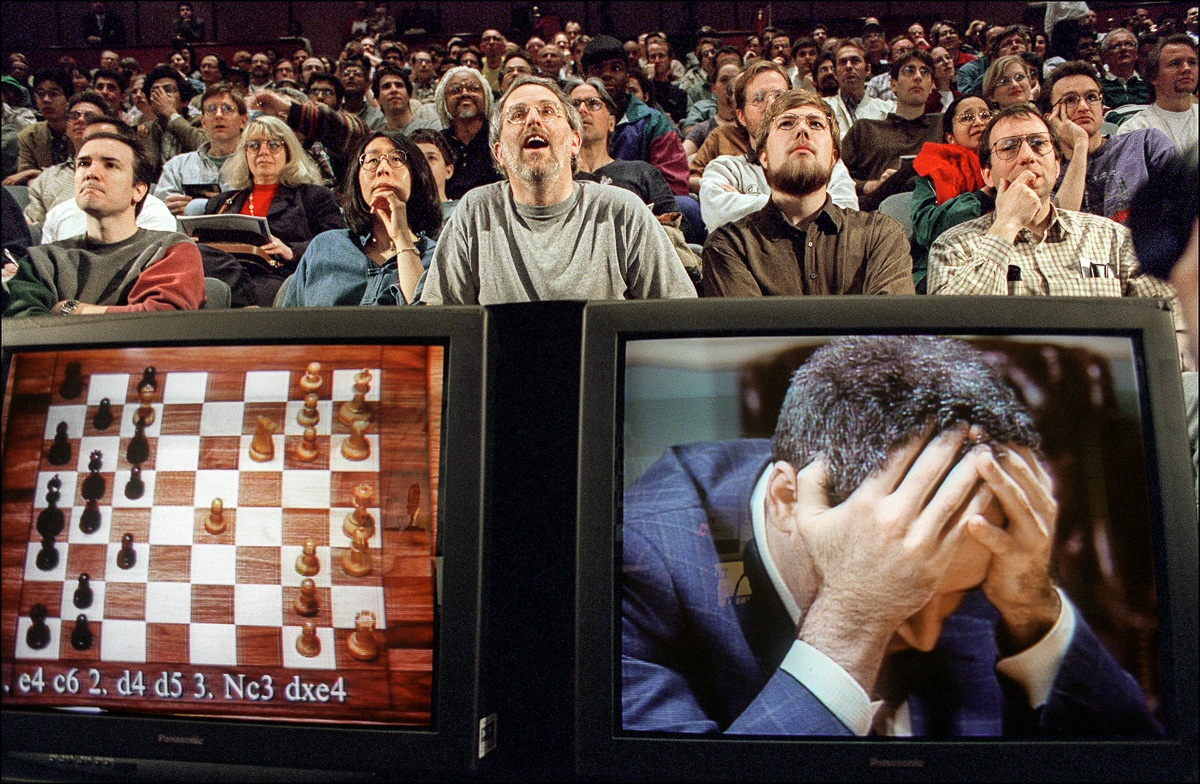
\includegraphics[width=0.8\textwidth]{figs/intro/deep_blue_2.png}

      棋迷在纽约通过电视观战。当日,卡斯帕罗夫在纽约再次负于深蓝,从而在当年的
      “人机大战”中以一胜二负三和的战绩败北。
    \end{column}
  \end{columns}
\end{frame}
